% CREATED BY DAVID FRISK, 2016
\chapter{Introduction}

In the beginning was the word and it was good. However, it is difficult to make computers understand natural languages. There are many different approaches that has been used to make this process easier. In this thesis we will focus on two such ways, both of which are meant to analyze the grammatical structure and syntax of a sentence.

% \begin{verbatim}
% - Kort om paradigmer
% - Kort om verktygen
% - Vad som är gjort
% - Vad som behöver göras

% Applications:
% - Let a computer understand human language
% - Allow the computer to do things with human writing
% - For example,
% -  - try to understand the meaning
% -  - make transformations on the writing (which?)
% -  - generate human language based on abstract knowledge
% \end{verbatim}

% Reliability and predictability are very important in many applications, for example law.


In rule-based Natural Language Processing (NLP) we want to be able to take a text and analyse it at a higher level and make transformations to it.
In order to do this, we first need a way to parse the text into a syntax tree, which describes the relationship between words in a sentence.



There are several different formalisms for describing sentences as trees, all with their own strengths and weaknesses.
The two we will be talking about here are Universal Dependencies (UD), which uses dependency trees, and Grammatical Framework (GF), which uses abstract syntax trees.

% \todo[inline]{Write more about the goal of the project and move the rest to background}

% \todo[inline]{Something general about rule-based NLG and NLP and computer grammars}

% TODO: Ta reda på vad UD används till

%  - dep trees, UD
\section{Dependency trees and Universal Dependencies}
A dependency tree is a tree structure that shows the grammatical relationship between words in a sentence. Each word becomes a node in the tree with the main verb as the root and the edges represents the relation and the direction of the dependency.

% For example in the sentence "John ate an apple", the word "ate" would become the root and "John" and "apple" would be direct children, where the arrow from "ate" to apple would be labeled as the subject relation while the arrow to "apple" would be labeled as the object. There would additionally be an arrow from "apple" to "an" which marks that "an" is a determiner for "apple".

% the root is black. cop stands copula, which is the word "is". nsubj stands for nominal subject and marks the subject of the sentence, that which is black. det stands for determiner, which answers which cat it is that is black

\todo[inline]{explain this picture}

\begin{figure}[H]
\centering
%% the cat is black
\setlength{\unitlength}{0.2mm}
\begin{picture}(205.0,90.0)
  \put(0.0,0.0){the}
  \put(37.0,0.0){cat}
  \put(83.0,0.0){is}
  \put(120.0,0.0){black}
  \put(0.0,15.0){{\tiny DET}}
  \put(37.0,15.0){{\tiny NOUN}}
  \put(83.0,15.0){{\tiny AUX}}
  \put(120.0,15.0){{\tiny ADJ}}
  \put(28.5,30.0){\oval(28.89189189189189,33.333333333333336)[t]}
  \put(14.054054054054054,35.0){\vector(0,-1){5.0}}
  \put(13.5,49.66666666666667){{\tiny det}}
  \put(88.5,30.0){\oval(79.3855421686747,66.66666666666667)[t]}
  \put(48.80722891566265,35.0){\vector(0,-1){5.0}}
  \put(73.5,66.33333333333334){{\tiny nsubj}}
  \put(111.5,30.0){\oval(28.89189189189189,33.333333333333336)[t]}
  \put(97.05405405405405,35.0){\vector(0,-1){5.0}}
  \put(96.5,49.66666666666667){{\tiny cop}}
  \put(135.0,90.0){\vector(0,-1){60.0}}
  \put(140.0,80.0){{\tiny root}}
\end{picture}
% \end{center}
\caption{The phrase ``the cat is black'' analyzed as a UD tree.} % Figure text below figure
\end{figure}

% Not mine: Universal Dependencies (UD) is a framework for representing the syntactic structure of natural language sentences. It is an annotation scheme that provides a universal set of part-of-speech tags and dependency labels that can be applied across different languages.

The specific standard for dependency trees that this paper is about is called Universal Dependencies (UD). UD is based on the idea of making a multilingual standard for dependency trees where the same set of tags can be used regardless of which language the sentence is written in.


% TODO: Robust för ogrammatiska meningar osv och ger alltid ett resultat

% \todo[inline]{Talk about the machine learning aspect of UD}

% One way to describe the structure of a sentence is through so-called dependency trees where the words in a sentence form a tree with one word is designated as the root and all the other words attach based on their relation to other words

% Using Dependency trees is a way of doing things \todo{write something here}

% Universal Dependencies is a specific dep tree thing for NLG \todo{and here}

% Universal Dependencies\cite{mcdonald-al-2013} (UD) is another grammar formalism which uses machine-learning for parsing, which allows it to use context more in order to guess which interpretation was intended. The training data is based on a large set of sentences, which have been manually tagged with labels and a tree structure.

%  - abstr trees, GF
\section{Abstract trees and Grammatical Framework}

Another way of describing the grammatical structure of a sentence is through abstract syntax trees, where instead of using words as the nodes in the tree, you use

% \todo[inline]{Write about abstract trees}
% \todo[inline]{Add an image}

Grammatical Framework\cite{ranta-2004} (GF) is a formalism for describing natural language grammars as code, which allows converting between natural language and a language-independent abstract syntax. It is split into a generic resource grammar that covers morphology and the language as a whole and application grammars for a more narrow domain which allows a more semantic abstract syntax. When you try to write a grammar that covers a very wide domain, you will often get an over-generating grammar where each sentence can be parsed in very many ways into many different trees, where usually only one is the intended way.

\begin{figure}[htb]
  \centering
  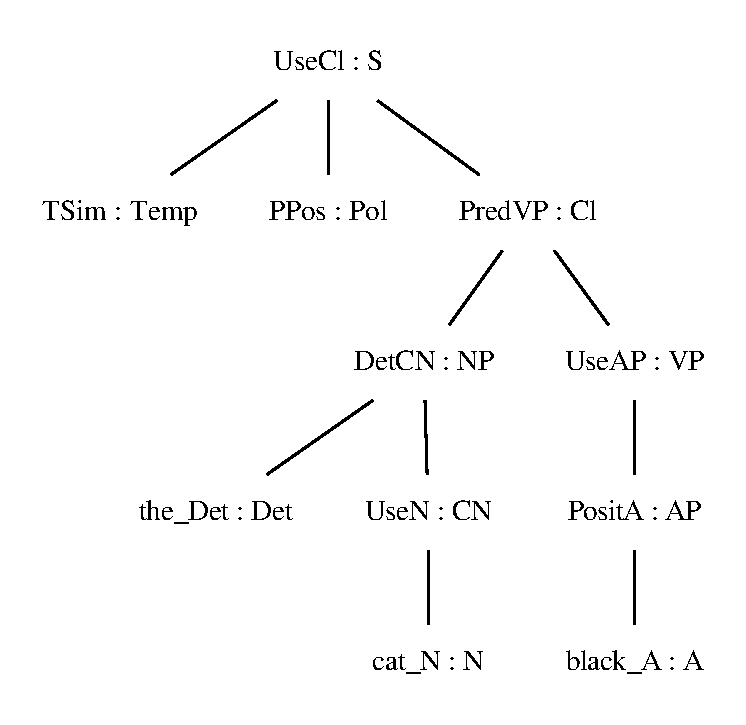
\includegraphics[width=0.5\linewidth]{thesis/figure/cat_is_black_gf.eps}
  \caption{The sentence ``The cat is black'' analyzed as a GF tree}
  \label{fig:universe}
\end{figure}


% NOTES:
% "The cat is black" vs "The cat is not black" corresponds to PPos vs PNeg
% ud2gf would have trouble differentiating between these because it's only in parameters
% Macros UseCl_NegCop and UseCl_Sim corresponds to the different versions
% These allows the information to be preserved, despite there not being any explicit GF function for the word ``not''
%
% Negative:
% UseCl_NegCop (StrNeg "not") (PredVP (DetCN_theSg (StrThe "the") (UseN cat_N)) (UseAP_Cop (StrCop "be") (PositA black_A)))
% Positive:
% UseCl_Sim (PredVP (DetCN_theSg (StrThe "the") (UseN cat_N)) (UseAP_Cop (StrCop "be") (PositA black_A)))

% #auxfun UseCl_Sim cl : Cl -> S = UseCl TSim PPos cl ; head
% #auxfun UseCl_Ant have cl : Have -> Cl -> S = UseCl TAnt PPos cl ; aux head
% #auxfun UseCl_NegSim do neg cl : Do -> Neg -> Cl -> S = UseCl TSim PNeg cl ; aux advmod head
% #auxfun UseCl_NegAnt have neg cl : Have -> Neg -> Cl -> S = UseCl TAnt PNeg cl ; aux advmod head
% #auxfun UseCl_NegCop neg cl : Neg -> Cl -> S = UseCl TSim PNeg cl ; advmod head

% #auxfun UseAP_Cop cop comp : Cop -> AP -> VP = UseAP comp ; cop head

% #auxcat Cop AUX
% #auxcat Do AUX
% #auxcat Have AUX
% #auxcat Neg PART

% Syncategorematic words:
% #word not not Polarity=Neg
% #word does  do  Mood=Ind|Number=Sing|Person=3|Tense=Pres|VerbForm=Fin
% #word is   be  Mood=Ind|Number=Sing|Person=3|Tense=Pres|VerbForm=Fin
% #word would would  VerbForm=Fin
% #word will  will VerbForm=Fin

% Syncategorematic lemmas:
% #lemma UseCl,UseQCl,ImpVP not Neg advmod head
% #lemma UseAP,UseAdv,UseNP be Cop cop head
% #lemma PredVP have Have aux head
% #lemma PredVP,ImpVP do Do aux head

%  - strengths and weaknesses
% 
\section{Differences between GF and UD}
% Strengths and weaknesses


% % Grammatical Framework has [some] advantages for [use-case], so it would be useful to be able to parse using UD and then get out a GF tree. A
GF is very strict when it comes to following grammar and spelling, which means that it will often refuse to parse sentences if they contain even the smallest error. UD on the other hand uses machine-learning to give some parse tree for all sentences regardless of how many errors they have.

While the machine-learning-based approach of UD allows it to guess the correct tree better for ambiguous sentences and allows it to handle grammatically incorrect sentences better, GF is much more capable when
it comes to performing transformations on the sentences, while maintaining correct morphology and grammar. This makes it attractive to parse sentences
using UD and then convert the parsed trees to GF trees in order to perform further transformations.


% Anteckningar

% UD har en massa manuellt annoterade träd som folk har tränat maskininlärningssystem på

% GF är mer strikt och kräver att grammatiken följs exakt och stavfel och små grammatikfel kommer inte

% UD är mer robust för fel och kommer alltid ge resultat oavsett om saker inte följs exakt och ger sin bästa gissning

% GF är mer exakt och förutsägbar, så buggar går bättre att anylysera och fixa

% Med GF kan man transformera meningar och träd på mycket fler sätt, till exempel kan ett påstående göras till en fråga bara genom att wrappa hela meningen med en MkQuestion funktion och då kommer automatiskt GF fixa alla morfosyntaktiska ändringar, så som att ändra ordföljd eller

% använder automatiskt rätt genus om man byter ut ett ord till ett annat

% abstrakt träd är oberoende av språk

% RGL beskriver morfosyntax för språk medan en applikationsgrammatik kan vara på högre nivå och ge mer ideomatiska översättningar och det beskrivs i termer av den abstrakta syntaxen för resursgrammatiken



% % Maybe mention the macros in the labels files

% % There exists a naive implementation based on a brute-force algorithm \cite{kolachina-ranta-2017}

% % Briefly describe and motivate the project, and convince the reader of the importance of the proposed thesis work.
% % A good introduction will answer these questions: Why is addressing these challenges significant for gaining new knowledge
% % in the studied domain? How and where can this new knowledge be applied?


\subsection{Useful synthesis between UD and GF}

\todo[inline]{explain about gf-ud, the old-old version, the new-old version and my developments on that}


There exists a proof-of-concept implementation of a tool for converting between the trees for GF and UD,
with the help of so-called labels-files which describe the mapping between UD labels and GF functions,
called gf-ud, which contains both a component for converting from UD to GF, called ud2gf\cite{kolachina-ranta-2017}\footnotemark[1]
and a component for converting from GF to UD, called gf2ud\cite{kolachina-ranta-2016}\footnotemark[1]. This work will focus on the ud2gf component.

\footnotetext[1]{These references apply to an older version of gf-ud, from before the one this thesis is based on. A part of the goal of this thesis is to document the later version in addition to documenting the changes made in the process of this thesis.}

% \todo{these references apply to an older version of gf-ud, from before the one I was working on. a part of the goal of this thesis is to document the old-new version that my changes was based on}

% The labels files can also contain macros, which allows constructing virtual GF functions during the translation from UD, which will be expanded to real GF functions at the end of the translation.
% These can, among other uses, be used to preserve information from the UD labels about subtrees, which can then be used at later points of the transformation to ensure that the desired GF tree is produced.

\subsection{Applications for the synthesis of UD and GF}

The gf-ud tool has been used for both translation and semantics\cite{ranta-al-2020}. %\todo{actually explain this}
Another application has been in concept alignment\cite{masciolini-ranta-2021}.
There has also been work using it for analysis of law text for the purpose of making a Controlled Natural Language for law\cite{listenmaa-etal-2021-towards}.



% Från mallen


% This chapter presents the section levels that can be used in the template.
%
% \section{Section levels}
% \autoref{tab:sections} presents an overview of the section levels that are used in this document. The number of levels that are numbered and included in the table of contents is set in the settings file \texttt{Settings.tex}. The levels are shown in Section \ref{Section_ref}.
%
% This is a new paragraph and should have proper parskip or indentation. Don't forget to cite your sources~\cite{listenmaa-etal-2021-towards}. % '~' becomes space which cannot line break.
%
% \begin{table}[h]
% \centering
% \caption{Section levels} % Table text above table.
% \begin{tabular}{ll} \hline
% Name & Command\\ \hline
% Chapter & \textbackslash\texttt{chapter\{\emph{Chapter name}\}}\\
% Section & \textbackslash\texttt{section\{\emph{Section name}\}}\\
% Subsection & \textbackslash\texttt{subsection\{\emph{Subsection name}\}}\\
% Subsubsection & \textbackslash\texttt{subsubsection\{\emph{Subsubsection name}\}}\\
% %Paragraph & \textbackslash\texttt{paragraph\{\emph{Paragraph name}\}}\\
% %Subparagraph & \textbackslash\texttt{paragraph\{\emph{Subparagraph name}\}}\\ \hline\hline
% \end{tabular}
% \label{tab:sections}
% \end{table}

% \section{Section} \label{Section_ref}
% \subsection{Subsection}
% \subsubsection{Subsubsection}
% \paragraph{Paragraph}
% \subparagraph{Subparagraph}
